\documentclass[]{article}
\usepackage{lmodern}
\usepackage{amssymb,amsmath}
\usepackage{ifxetex,ifluatex}
\usepackage{fixltx2e} % provides \textsubscript
\ifnum 0\ifxetex 1\fi\ifluatex 1\fi=0 % if pdftex
  \usepackage[T1]{fontenc}
  \usepackage[utf8]{inputenc}
\else % if luatex or xelatex
  \ifxetex
    \usepackage{mathspec}
    \usepackage{xltxtra,xunicode}
  \else
    \usepackage{fontspec}
  \fi
  \defaultfontfeatures{Mapping=tex-text,Scale=MatchLowercase}
  \newcommand{\euro}{€}
\fi
% use upquote if available, for straight quotes in verbatim environments
\IfFileExists{upquote.sty}{\usepackage{upquote}}{}
% use microtype if available
\IfFileExists{microtype.sty}{%
\usepackage{microtype}
\UseMicrotypeSet[protrusion]{basicmath} % disable protrusion for tt fonts
}{}
\usepackage[margin=1in]{geometry}
\ifxetex
  \usepackage[setpagesize=false, % page size defined by xetex
              unicode=false, % unicode breaks when used with xetex
              xetex]{hyperref}
\else
  \usepackage[unicode=true]{hyperref}
\fi
\hypersetup{breaklinks=true,
            bookmarks=true,
            pdfauthor={Andrea Fernández},
            pdftitle={Proyecto 3: Orquestación},
            colorlinks=true,
            citecolor=blue,
            urlcolor=blue,
            linkcolor=magenta,
            pdfborder={0 0 0}}
\urlstyle{same}  % don't use monospace font for urls
\setlength{\parindent}{0pt}
\setlength{\parskip}{6pt plus 2pt minus 1pt}
\setlength{\emergencystretch}{3em}  % prevent overfull lines
\setcounter{secnumdepth}{5}

%%% Use protect on footnotes to avoid problems with footnotes in titles
\let\rmarkdownfootnote\footnote%
\def\footnote{\protect\rmarkdownfootnote}

%%% Change title format to be more compact
\usepackage{titling}
\setlength{\droptitle}{-2em}
  \title{Proyecto 3: Orquestación}
  \pretitle{\vspace{\droptitle}\centering\huge}
  \posttitle{\par}
  \author{Andrea Fernández}
  \preauthor{\centering\large\emph}
  \postauthor{\par}
  \predate{\centering\large\emph}
  \postdate{\par}
  \date{30/05/2015}


\usepackage{float}
\usepackage{morefloats}
\usepackage[spanish]{babel}
\usepackage{graphicx}
\usepackage{tcolorbox}
\usepackage{rotating}
\usepackage{longtable}
\usepackage{colortbl}
%\usepackage{natbib}
%\newenvironment{scaleb}{ \scalebox{0.4}{} {} }
%\newenvironment{scaleb}{ \tiny{} }
% biber
\usepackage[autostyle]{csquotes}

\usepackage[
    backend=biber,
    style=authoryear-icomp,
    sortlocale=de_DE,
    natbib=true,
    url=false,
    doi=true,
    eprint=false
]{biblatex}
\addbibresource{bibliografia.bib}

\usepackage[]{hyperref}
\hypersetup{
% Turn on this if you prefer to have links colored instead of marked with squares
colorlinks = true,
linkcolor = black,
urlcolor = blue,
citecolor = black,
% pdfpagemode = UseNone
}

\renewcommand\figurename{Figura}
\renewcommand\tablename{Tabla}

\newenvironment{myexampleblock}[1]{%
    \tcolorbox[beamer,%
    noparskip,breakable,
    colback=LightGreen,colframe=DarkGreen,%
    colbacklower=LimeGreen!75!LightGreen,%
    title=#1]}%
    {\endtcolorbox}

\newenvironment{myalertblock}[1]{%
    \tcolorbox[beamer,%
    noparskip,breakable,
    colback=LightCoral,colframe=DarkRed,%
    colbacklower=Tomato!75!LightCoral,%
    title=#1]}%
    {\endtcolorbox}

\newenvironment{myblock}[1]{%
    \tcolorbox[beamer,%
    noparskip,breakable,
    colback=LightBlue,colframe=DarkBlue,%
    colbacklower=DarkBlue!75!LightBlue,%
    title=#1]}%
    {\endtcolorbox}


\begin{document}

\maketitle


{
\hypersetup{linkcolor=black}
\setcounter{tocdepth}{3}
\tableofcontents
}
\pagebreak

\section{Introducción}\label{introduccion}

Generalmente se dice que el procesamiento a gran escala debe cumplir las
tres V's: Volumen, Velocidad y Variedad. La necesidad de procesar
información a gran escala de forma muy rápida ha llevado a la creación
de una gran variedad de soluciones con diferentes características, lo
anterior ha permitido que en la actualidad se pueda disponer de diversas
herramientas para la implementación de procesos que impliquen el
análisis de grandes cantidades de datos. Cada una de las herramientas
desarrolladas hasta la actualidad cuentan con ventajas y desventajas que
deben ser analizadas dependiendo el tipo de proyecto y análisis que se
quiera desarrollar, lo anterior permitirá identificar la herramienta que
mejor se adapte a las necesidades del proyecto a desarrollar. A
continuación se describen las características de cada una de las
herramientas utilizadas en el desarrollo de nuestro proyectos y la
implementación que se realizó.

\section{Pipeline de datos}\label{pipeline-de-datos}

\subsection{Objetivo}\label{objetivo}

Implementar el flujo para la base de datos de \textbf{GDELT}:

\begin{itemize}
\itemsep1pt\parskip0pt\parsep0pt
\item
  Obtención:

  \begin{itemize}
  \itemsep1pt\parskip0pt\parsep0pt
  \item
    Crawler
  \item
    Identificar si hay nueva información
  \item
    Bajar a zip
  \item
    Guardar en disco
  \item
    Descomprimir
  \end{itemize}
\item
  Limpieza:

  \begin{itemize}
  \itemsep1pt\parskip0pt\parsep0pt
  \item
    Revisar columnas
  \item
    Quitar columnas no requeridas
  \item
    Estructurar las columnas en un orden apropiado
  \item
    Realizar proceso de normalización de datos (e.g.~fechas a UTC)
  \item
    Enviar a un archivo de texto
  \end{itemize}
\item
  Manipulación:

  \begin{itemize}
  \itemsep1pt\parskip0pt\parsep0pt
  \item
    Detectar que se escribió un archivo de texto y triggerear la subida
    al HDFS
  \item
    Realizar un proceso de analítica que actualice la información
  \item
    Tener una base de datos para shiny actualizada
  \end{itemize}
\end{itemize}

\subsection{Herramientas a utilizar}\label{herramientas-a-utilizar}

\begin{enumerate}
\def\labelenumi{\arabic{enumi}.}
\itemsep1pt\parskip0pt\parsep0pt
\item
  Sistema de carpetas / configuración / docker
\item
  Flume
\item
  Luigi
\item
  Spark
\item
  Sqoop
\item
  Hive/Impala
\end{enumerate}

\subsection{Implementación}\label{implementacion}

\begin{figure}[H]
\centering
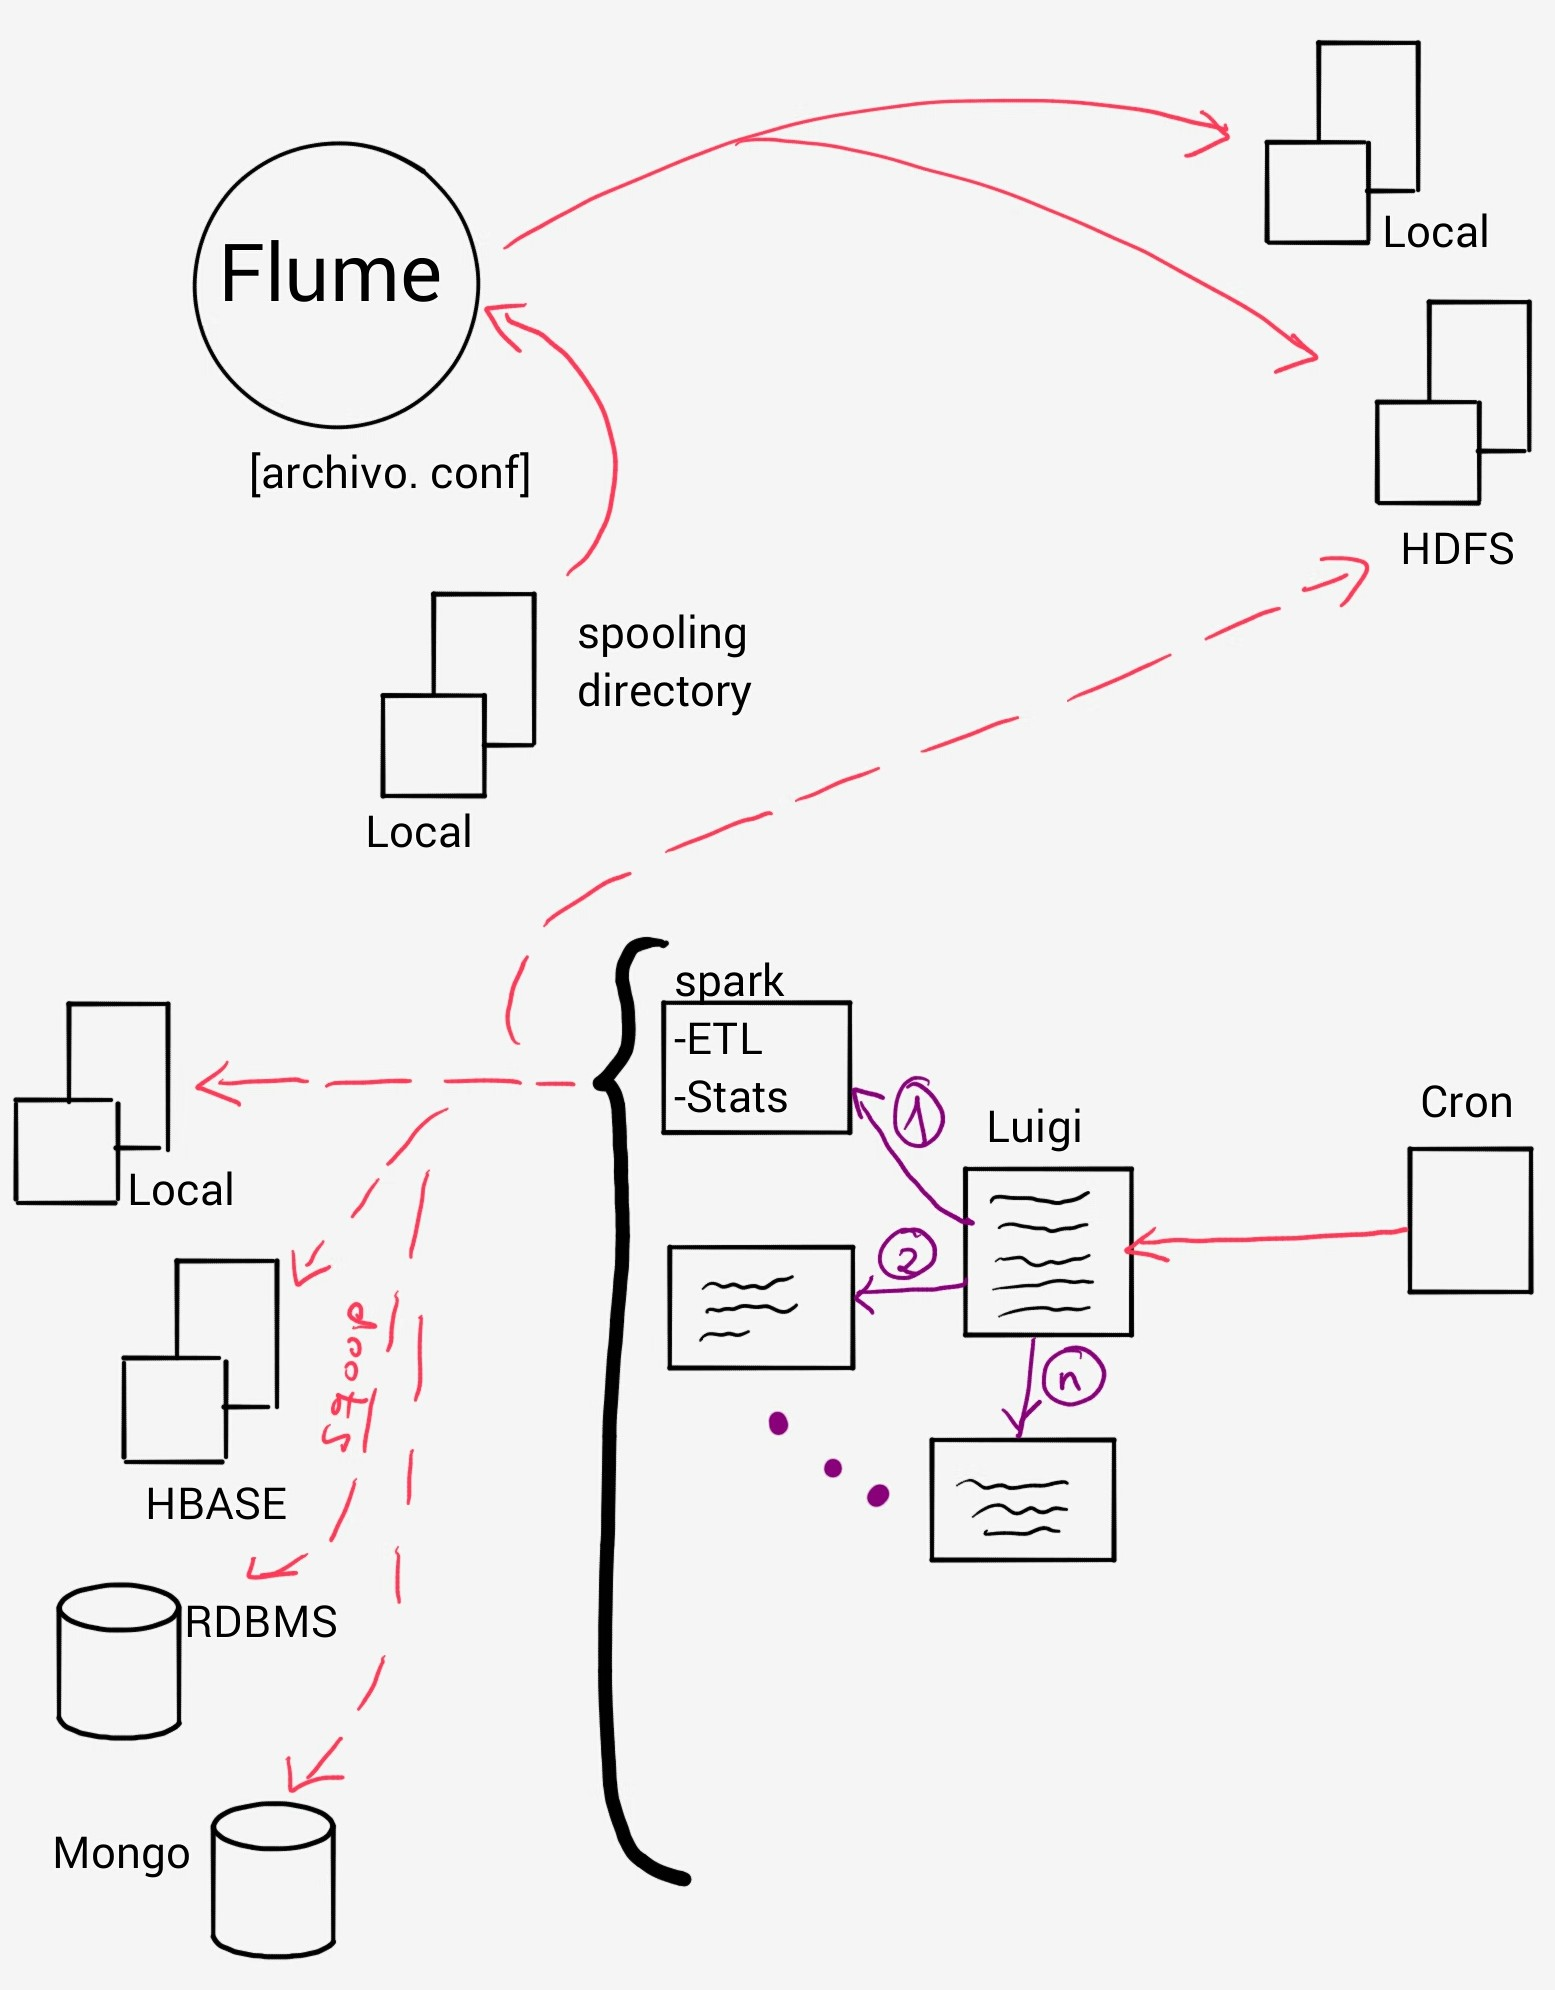
\includegraphics[width=0.8 \textwidth]{img/arquitectura.jpg}
\caption{Flujo de datos implementado.}
\end{figure}

\section{Configuración}\label{configuracion}

\subsection{Docker}\label{docker}

Se utiliza el docker de clase disponible en
\url{https://registry.hub.docker.com/u/nanounanue/docker-hadoop/}.

\section{Apache Flume}\label{apache-flume}

\subsection{¿Qué es?}\label{que-es}

\texttt{Flume} es un sistema distribuido y seguro para recoger, agregar
y mover grandes volúmenes de datos provenientes de logs desde distintas
fuentes a un almacén de datos centralizado. La arquitectura de
\texttt{Flume} se puede dividir en seis partes: - Fuente externa. Se
trata de la aplicación o mecanismo, como un servidor web o una consola
de comandos desde la cual se generan eventos de datos que van a ser
recogidos por la fuente. - Fuente. Una fuente es un componente que se
encarga de recoger eventos desde la fuente externa y pasárselos
transaccionalmente al canal. - Canal. Un canal es otro componente que
actuará de almacén intermedio entre la fuente y el sumidero. La fuente
será la encargada de escribir los datos en el canal y permanecerán en él
hasta que el sumidero u otro canal los consuman. - Sumidero. Este
componente será el encargado de recoger los datos desde el canal
intermedio dentro de una transacción y de moverlos a un repositorio
externo. - Repositorio externo. Nos sirve para almacenar en un sistema
de ficheros como puede ser HDFS. - Interceptores. Serán una parte
transversal de la arquitectura y podrán ser relacionados cuando ocurran
distintos tipos de eventos en el flujo. Los interceptores podrán
procesar los datos y añadirles la lógica que se necesite.

\subsection{¿Para qué se utiliza?}\label{para-que-se-utiliza}

El uso de \texttt{Flume} no sólo se limita a la agregación de datos
desde logs. Debido a que las fuentes de datos son configurables,
\texttt{Flume} permite ser usado para recoger datos desde eventos
ligados al tráfico de red, redes sociales, mensajes de correo
electrónico a casi cualquier tipo de fuente de datos posibles. Flume
soporta cuatro tipos de protocolos para leer datos:

\begin{itemize}
\itemsep1pt\parskip0pt\parsep0pt
\item
  Avro
\item
  Thrift
\item
  Syslog
\item
  Netcat
\end{itemize}

Los distintos componentes de un flujo de eventos en Flume deberán
implementar algún tipo de cliente o servidor que sea compatible con
alguno de los cuatro protocolos anteriores.

Al tratarse de una arquitectura modular podemos concatenar distintos
flujos para hacer un sistema más complejo como puede verse en la
siguiente imagen:

\subsection{Ventajas y desventajas}\label{ventajas-y-desventajas}

Sus principales ventajas:

\begin{itemize}
\itemsep1pt\parskip0pt\parsep0pt
\item
  Permite mover, de manera agregada y eficiente, grandes cantidades de
  datos de resgistro de muchas fuentes diferentes a Hadoop.
\item
  Permite usar como entrada de datos un gran número de fuentes de
  eventos.
\item
  Flume está pensado para procesos en streaming (intentando llegar a
  algo cercano a Real-time).
\item
  Permite definir el flujo de ejecución de manera que podemos indicar
  los componentes por los que va pasando nuestra ejecución. Sus
  principales desventajas:
\item
  cada nodo puede engrentar algunos problemas de rendimiento cuando la
  capacidad de procesamiento de datos del nodo se excede de forma
  inesperada debido a la enorme cantidad de carga de trabajo.
\item
  Si la cantidad de datos transmitidos al nodo es demasiado pequño en
  comparación con su capacidad de procedamiento de datos, el nodo puede
  llegar a ser subtutilizado.`
\end{itemize}

\subsection{Implementación}\label{implementacion-1}

\begin{figure}[H]
\centering
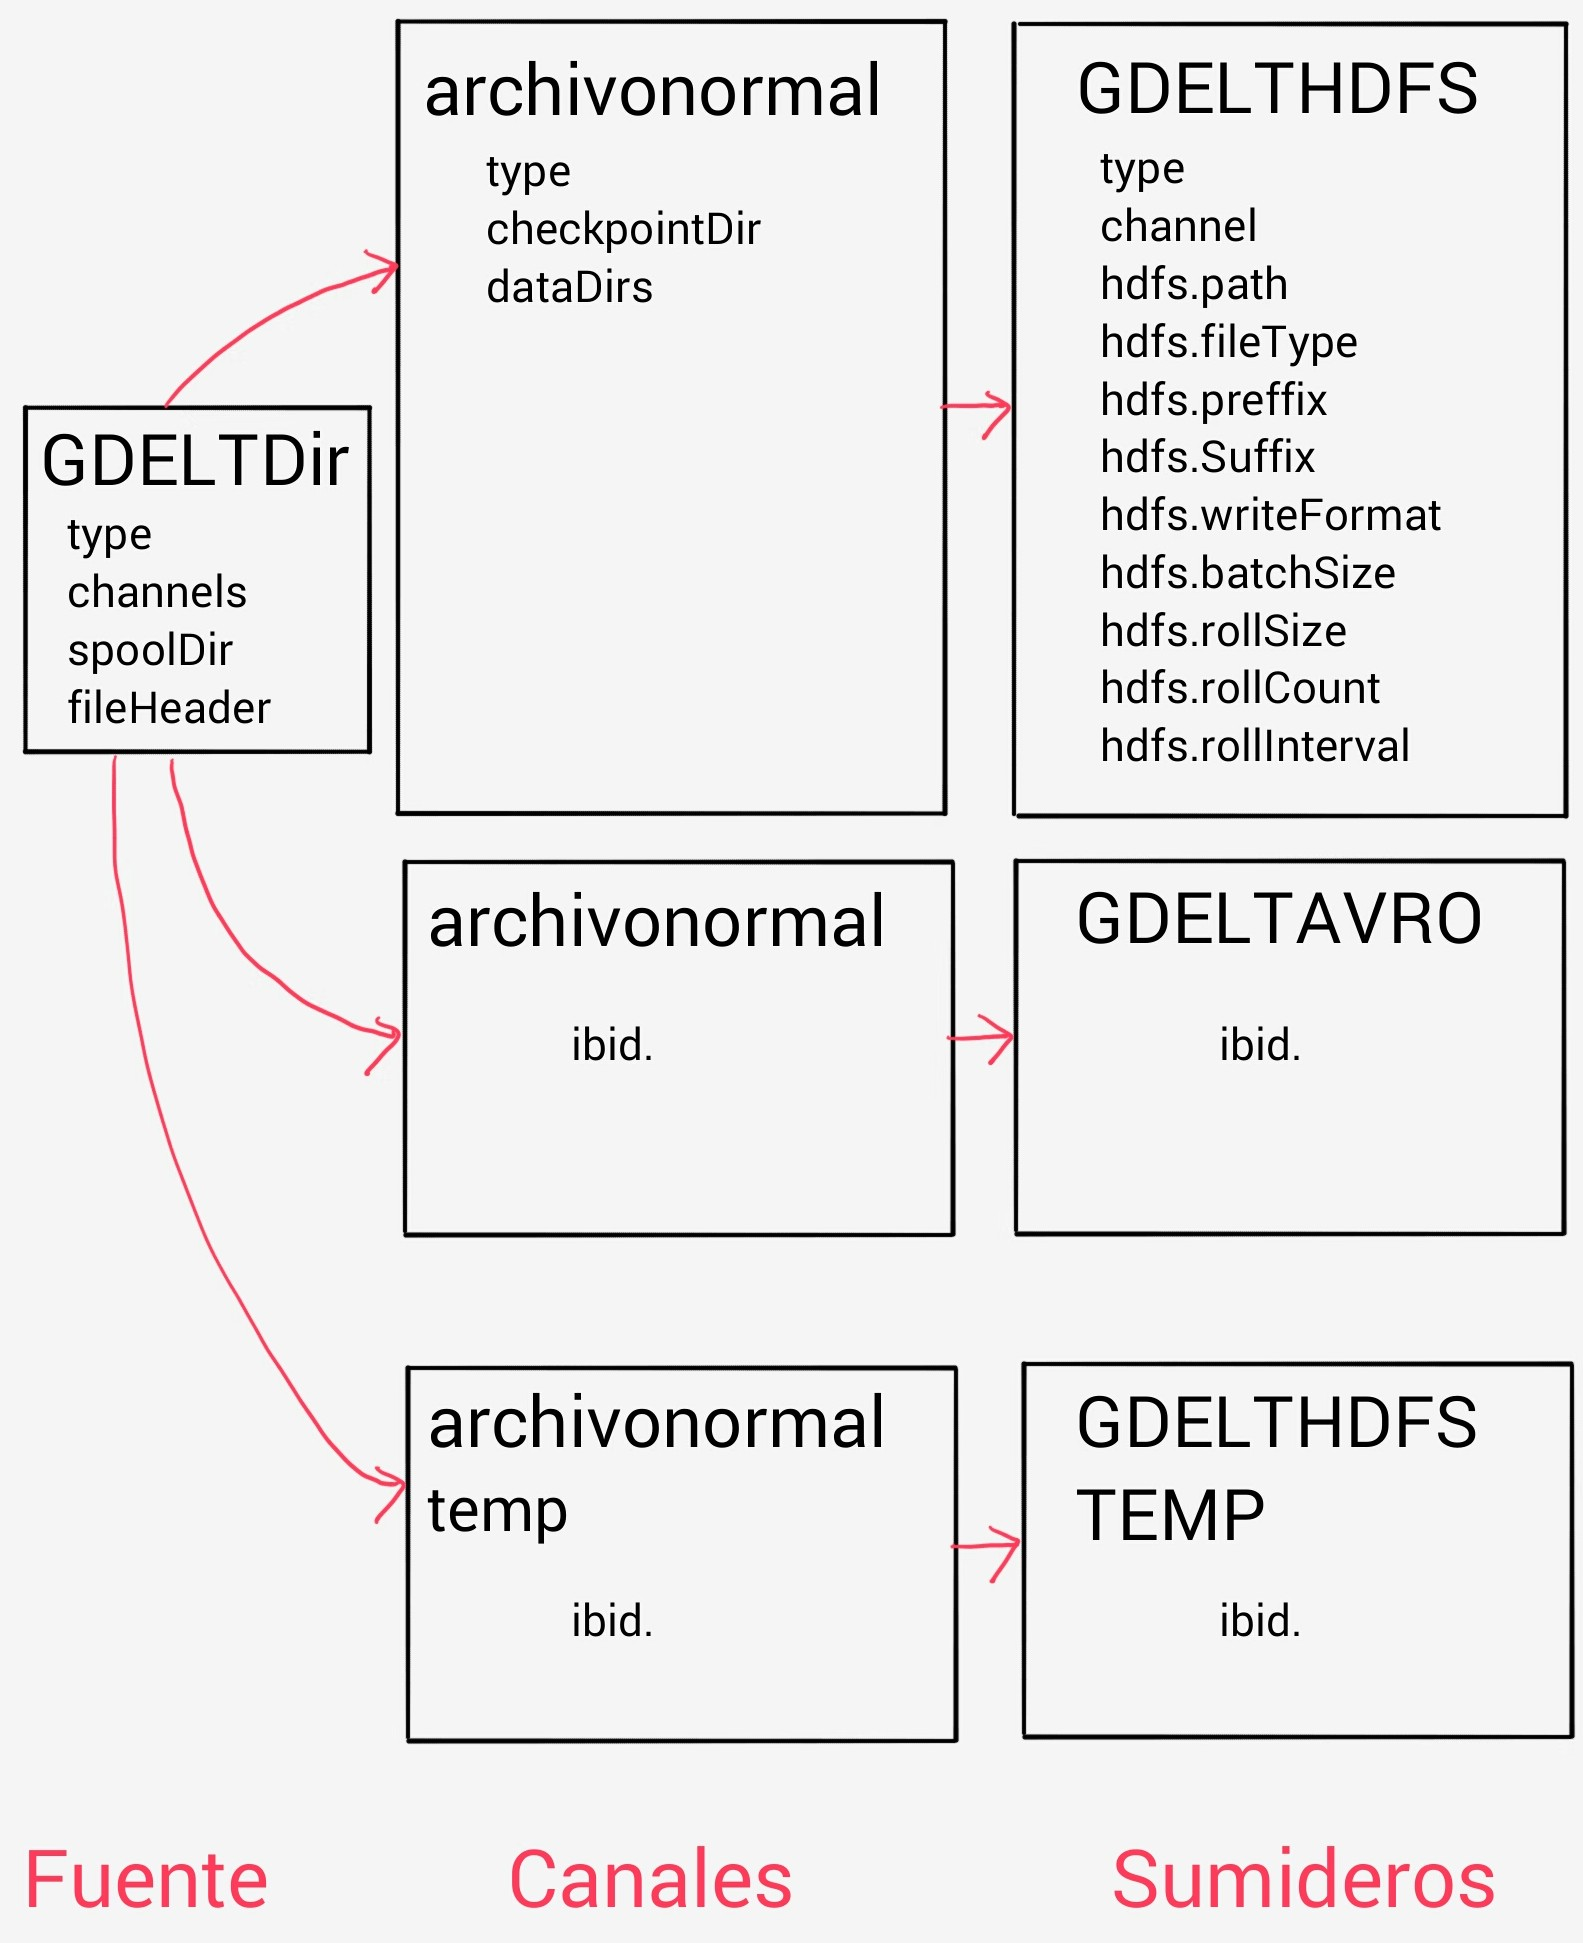
\includegraphics[width=0.8 \textwidth]{img/flume.jpg}
\caption{Fuente, canales y sumideros definidos en \emph{gdelt\_flume\_agent.conf}.}
\end{figure}

\section{Spark}\label{spark}

\subsection{¿Qué es?}\label{que-es-1}

\texttt{Spark} es una plataforma de computación de código abierto para
análisis y procesos avanzados. Desde su principio \texttt{Spark} fue
diseñado para soportar en memoria algoritmos iterativos que se pudieran
desarrollar sin escribir un conjunto de resultados cada vez que
procesaba un dato. Esta habilidad para mantener todo en memoria es una
técnica de computación de alto rendimiento aplicado al análisis
avanzado.

\subsection{¿Para qué se utiliza?}\label{para-que-se-utiliza-1}

\texttt{Spark} es utilizado para implementar análisis avanzados, cuenta
con un \texttt{framework} que incluye:

\begin{itemize}
\itemsep1pt\parskip0pt\parsep0pt
\item
  La librería Mlib para implementar funciones para Machine Learning.
\item
  El motor de gráficos GraphX.
\item
  \texttt{Spark Streaming} para procesar en tiempo real grandes
  cantidades de datos.
\item
  \texttt{Sparck SQL} para procesar consultas en \texttt{SQL}.
\end{itemize}

Esta plataforma asegura a los usuarios la consistencia en los resultados
a través de distintos tipos de análisis.

\subsection{Ventajas y desventajas}\label{ventajas-y-desventajas-1}

Sus principales ventajas:

\begin{itemize}
\itemsep1pt\parskip0pt\parsep0pt
\item
  Capacidad de procesamiento en memoria, \texttt{Spark} tiene
  velocidades de procesamiento hasta 100 veces más rápidas que las
  conseguidas utilizando \texttt{MapReduce}.
\item
  Esquema de computación más flexible que \texttt{MapReduce}.
\item
  Se puede descargar y ejecutar desde un ordenador personal.
\item
  Actualmente \texttt{Spark} es apoyado comercialmente por
  \texttt{Cloudera}, \texttt{Hortonworks} y \texttt{DataBricks}.
\item
  Se pueden desarrollar aplicaciones en \texttt{Spark} utilizando
  \texttt{Java}, \texttt{Scala}, \texttt{Phyton} y \texttt{R}.
\item
  Unificación del streaming en tiempo real.
\item
  Permite integrarse con una gran cantidad de fuentes y repositorios de
  datos.
\end{itemize}

Sus principales desventajas:

\begin{itemize}
\itemsep1pt\parskip0pt\parsep0pt
\item
  Consume mucha memoria
\item
  Solo soporta los sistemas de archivo a través de \texttt{HDFS}
\end{itemize}

\subsection{Implementación}\label{implementacion-2}

\section{Sqoop}\label{sqoop}

\subsection{¿Qué es?}\label{que-es-2}

\texttt{Sqoop} es una librería que permite importar datos desde un
almacenamiento de datos estructurado, como una base de datos relacional,
a \texttt{Hadoop}. \texttt{Sqoop} también permite importar datos a otras
bases de datos como \texttt{Hive} o \texttt{HBase}.

\subsection{¿Para qué se utiliza?}\label{para-que-se-utiliza-2}

\texttt{Sqoop} suministra una herramienta desde línea de comando a
través de la cual se puede realizar todo el proceso de importación y
exportación de datos desde una base de datos relacional a un sistema de
ficheros distribuidos y viceversa.

\subsection{Ventajas y desventajas}\label{ventajas-y-desventajas-2}

Sus principales ventajas:

\begin{itemize}
\itemsep1pt\parskip0pt\parsep0pt
\item
  Agiliza y facilita el movimiento de datos dentro y fuera de Hadoop.
\item
  Sqoop está enfocado a bases de datos relacionales.
\item
  Sqoop utiliza durante su ejecucción el paradigma MapReduce. Lo que
  permite procesar la información de manera paralela en procesos batch.
\item
  Lanza directamente una o varias tareas MapReduce para procesar los
  datos.
\end{itemize}

Sus principales desventajas:

\begin{itemize}
\itemsep1pt\parskip0pt\parsep0pt
\item
  Solamente realiza la validación a los datos copiados de una sola tabla
  en \texttt{HDFS}.
\end{itemize}

\subsection{Implementación}\label{implementacion-3}

\section{Orquestación vía Luigi}\label{orquestacion-via-luigi}

\subsection{¿Qué es?}\label{que-es-3}

\texttt{Luigi} es una herramienta de generación de \texttt{workflows} y
\texttt{pipelines} de trabajo. Permite definir distintos tipos de
tareas, así como las dependencias de ejecución entre ellas, además de
disponer de una interfaz de visualización para comprobar el estado de la
ejecución y de la finalización del \texttt{workflow} completo. Está
escrito en \texttt{Python}, y tiene plantillas predefinidas para varios
tipos de tareas.

\subsection{¿Para qué se utiliza?}\label{para-que-se-utiliza-3}

Permite gestionar la dependencia entre tareas mediante una serie de
funciones que se deben reescribir. Las más importantes son las
siguiente:

\begin{itemize}
\itemsep1pt\parskip0pt\parsep0pt
\item
  Run. Esta función contendrá el código principal de la tarea que se
  desea ejecutar.
\item
  Requires. La función requires establece la relación de dependencia
  entre dos tareas.
\item
  Output. La función output especifica la referencia al contenido que la
  tarea genera. Si se lanza varias veces el mismo \texttt{workflow},
  antes de ejecutar cada una de las tareas, \texttt{Luigi} comprobará
  que no exista la referencia marcada en el \texttt{output}. En caso de
  que exista, la tarea se marcará como completada y pasará a la
  siguiente.
\end{itemize}

\subsection{Ventajas y desventajas}\label{ventajas-y-desventajas-3}

\subsection{Implementación}\label{implementacion-4}

\begin{figure}[H]
\centering
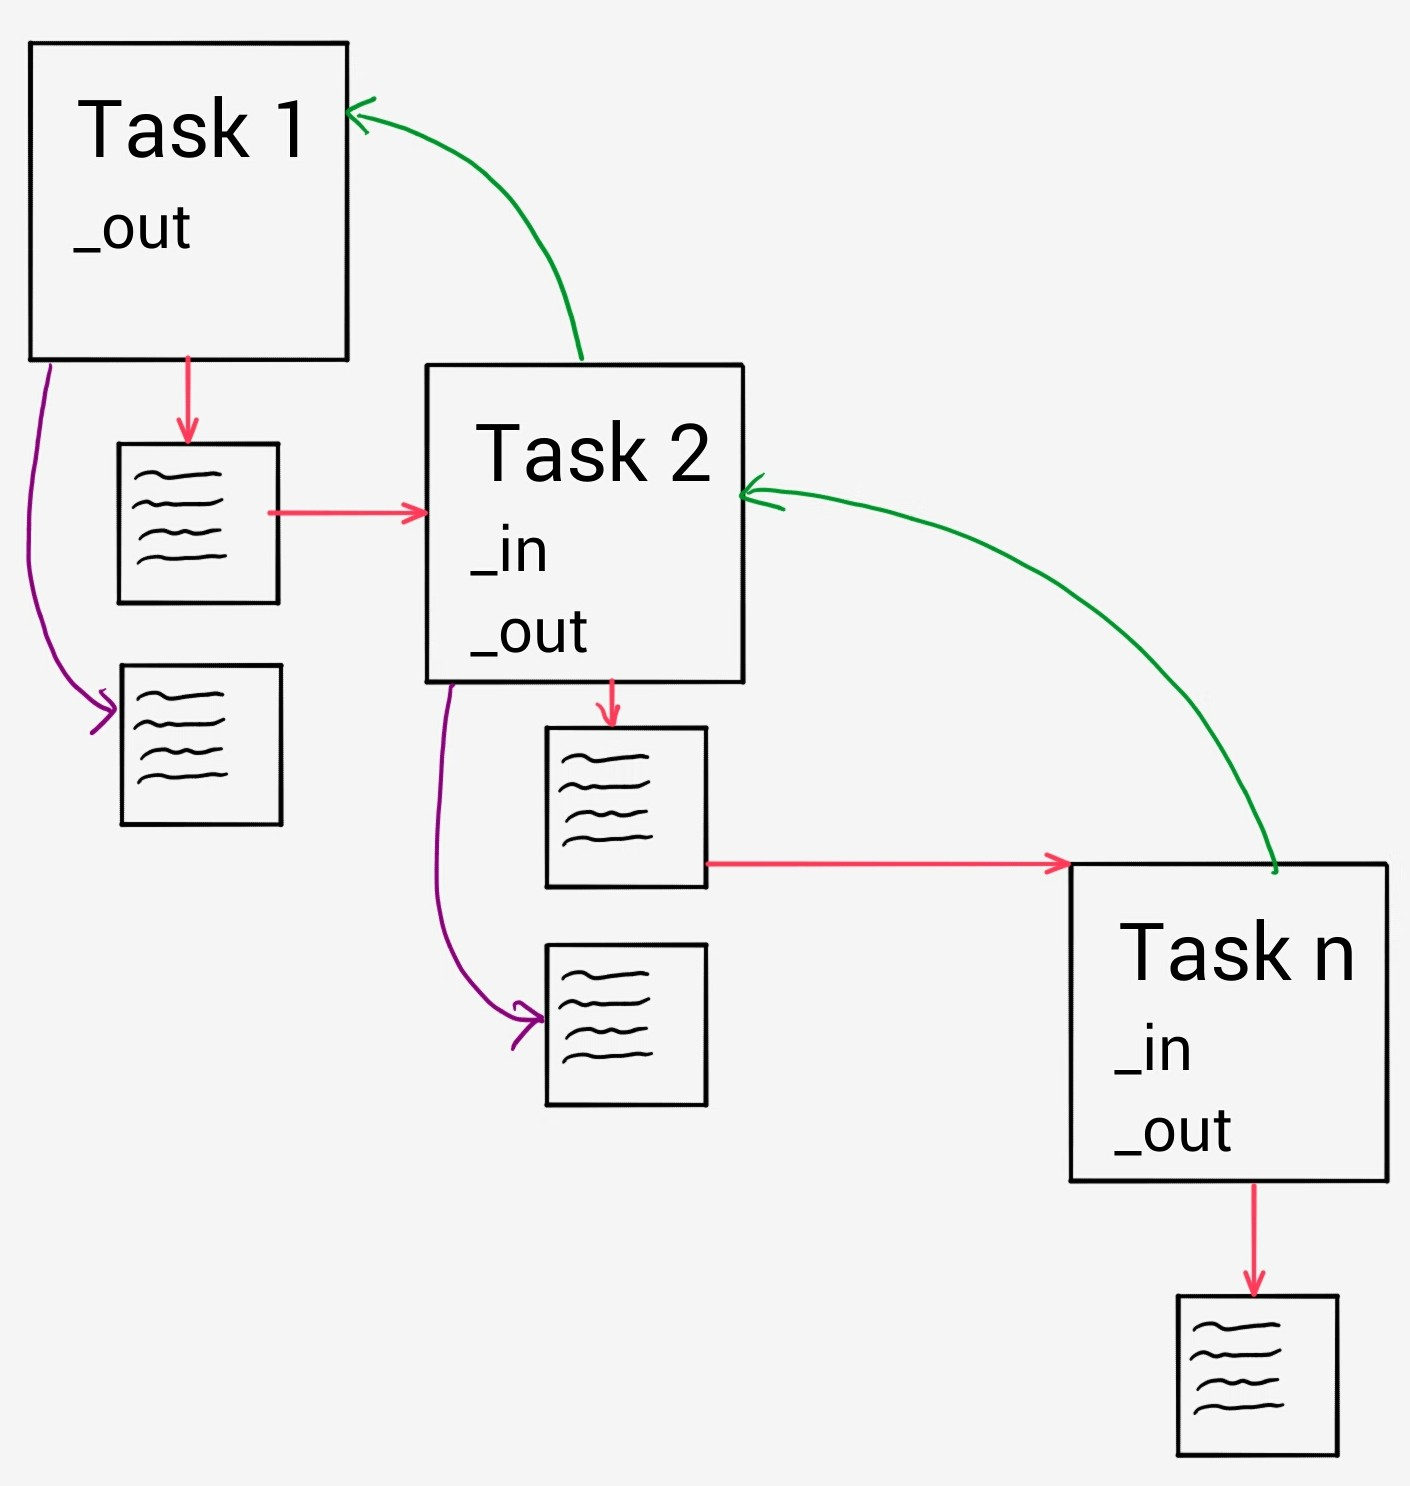
\includegraphics[width=0.8 \textwidth]{img/luigi.jpg}
\caption{Esquema de las tareas implementadas en \emph{orquestador\_gdelt.py}.}
\end{figure}

\section{Hive}\label{hive}

\subsection{¿Qué es?}\label{que-es-4}

\texttt{Hive} es un sistema de almacén de datos que facilita el manejo
sencillo de datos, consultas ad-hoc, y el análisis de grandes conjuntos
de datos almacenados en sistemas de ficheros compatibles con
\texttt{Hadoop}.

Algunas de las principales características de \texttt{Hive} y de su
lenguaje \texttt{HiveQL} son las siguientes:

\begin{itemize}
\itemsep1pt\parskip0pt\parsep0pt
\item
  \texttt{HiveQL} es un lenguaje tipo \texttt{SQL} que permite realizar
  consultas de grandes volúmenes de datos almacenados en un sistema de
  ficheros compatible con \texttt{Hadoop}.
\item
  Las consultas realizadas desde \texttt{HiveQL} se ejecutan siguiendo
  el modelo \texttt{MapReduce}.
\item
  \texttt{Hive} necesita almacenar metadatos y los esquemas de datos
  mediante un servicio metastore.
\item
  El programador no necesita \texttt{HiveQL} ningún maper o reducer lo
  que agiliza el desarrollo. \texttt{Hive} se encarga de traducir la
  consulta escrita con \texttt{HiveQL} en tareas \texttt{MapReduce}.
\item
  \texttt{Hive} permite que el programador pudiera escribir sus propios
  mares y reduces si fuera necesario
\item
  \texttt{HiveQL} no permite inserción, actualización o borrado de datos
  a nivel de registro. Tampoco dota de transaccionalidad a sus
  consultas.
\item
  Permite crear tablas y insertar datos que están almacenados en el
  sistema de ficheros de \texttt{Hadoop}.
\item
  La latencia de las consultas suele ser mayor que las realizadas en las
  bases de datos relacionales debido a la inicialización de
  \texttt{MapReduce}.
\item
  Schema on read vs schema on write. A diferencia de las bases de datos
  relacionales que garantizan que el \texttt{Schema} se cumple cuando se
  inserta un registro, \texttt{Hive} no garantiza esto aunque intenta
  garantizar el esquema en las lecturas.
\end{itemize}

\subsection{¿Para qué se utiliza?}\label{para-que-se-utiliza-4}

Hive provee un mecanismo para dotar de estructura en los datos y
realizar consultas sobre los mismos con el lenguaje tipo SQL llamado
HiveQL. Al mismo tiempo este lenguaje también permite a los
programadores de \texttt{MapReduce} incluir sus propios mappers y
reducers cuando no sea conveniente o eficiente expresar esta lógica con
HiveQL.

\subsection{Ventajas y desventajas}\label{ventajas-y-desventajas-4}

Se recomienda utilizar \texttt{Hive} para el procesamiento secuencial de
grandes archivos de datos multi-estructurados. Las principales ventajas
de \texttt{Hive} son:

\begin{itemize}
\itemsep1pt\parskip0pt\parsep0pt
\item
  Su capacidad de mejorar la simplicidad y la rapidez del desarrollo de
  \texttt{MapReduce}.
\item
  Hace más sencillo el procesamiento de archivos relacionados entre sí.
\item
  Utiliza queries similares a \texttt{SQL}.
\end{itemize}

Las principales desventajas de \texttt{Hive} son:

\begin{itemize}
\itemsep1pt\parskip0pt\parsep0pt
\item
  No está completamente aislado del sistema de archivos subyacente, esto
  implica que con frecuencia el usuario requiere ayuda del optimizador
  con construcciones del lenguaje para procesar consultas más complejas.
\item
  No puede sustituir a la funcionalidad, facilidad de uso, el
  rendimiento y la madurez de un \texttt{DBMS}.
\end{itemize}

\subsection{Implementación}\label{implementacion-5}

\section{Conclusiones}\label{conclusiones}

\section{Bibliografía}\label{bibliografia}

\end{document}
